\documentclass{article}
\usepackage{graphicx, caption, subcaption}
\usepackage{blindtext}
\usepackage{actuarialsymbol}
\usepackage{xcolor}
\definecolor{ultramarine}{RGB}{0,85,180}
\usepackage[a4paper,total={170mm,247mm},top=2.5cm]{geometry}
\usepackage{fancyhdr}
\usepackage{booktabs}
\usepackage{cellspace}
\usepackage{siunitx} %number rounding
\usepackage{numprint}

\setlength\cellspacetoplimit{10pt}
\setlength\cellspacebottomlimit{2pt}
\pagestyle{fancy}
\graphicspath{{./}}
\lhead{
\includegraphics[width=0.28\textwidth]{logo.png}}
\setlength{\headheight}{1cm} % Set header height
\setlength{\footskip}{1cm} % Set footer height
\fancyfoot[R]{\large{\textbf{\textcolor{red}{Rigaku confidential}}}}
\fancyfoot[C]{\thepage} % Align page number to the page center

% Define variable parameters 
\newcommand{\SerialNumber}{\text{037}}
\newcommand{\Optics}{\text{037-066}}
\newcommand{\OpticsType}{\text{C0-06-19}}
\newcommand{\Fokus}{\text{22.85}}
\newcommand{\FokusTime}{\text{8}}
\newcommand{\CircleTime}{\text{150}}
\newcommand{\Author}{\text{Veronika Marsikova}}
\newcommand{\Customer}{\text{BRU}}
\newcommand{\ReportName}{\text{TEST REPORT}}

\rhead{\large{\textbf{\textcolor{ultramarine}{\Optics{}}}}}

\title{\textbf{\textcolor{ultramarine}{\Optics{} (C0-06-19)}}}
\date{\textbf{\textcolor{ultramarine}{\ReportName{}}}}

\begin{document}

 \maketitle
 \thispagestyle{fancy} % Přidáváme fancy styl na titulní stranu
\captionsetup[subfigure]{singlelinecheck=off, justification=centering}

\begin{figure}[ht]
    \begin{center}
    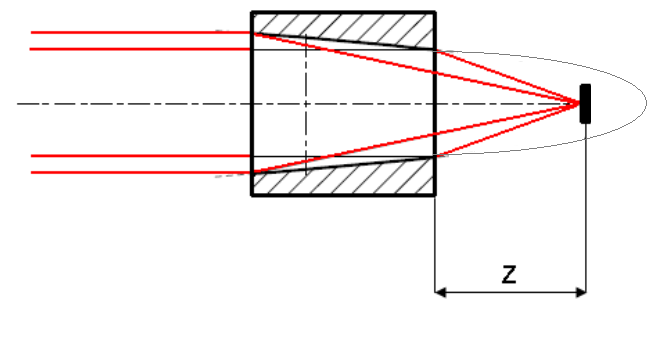
\includegraphics[width= 7 cm]{optics_parabola.png}
    \end{center}
    \label{fig:optika}
\end{figure}

%{\textcolor{red}{Bóďa - lépe to nešlo}}

\textbf{\textcolor{ultramarine}{General:}}\\
\begin{center}
    	\renewcommand{\arraystretch}{1.15} % Násobek výchozí výšky řádků
    \begin{tabular}{|p{7cm}|p{7cm}|}
\hline
Tested by:&			\Author{}\\	\hline
Date:&				\today\\	\hline
Serial number:&		\SerialNumber{}\\	\hline
Product number:&	\Optics{}\\	\hline
Customer:&			\Customer{}\\
&						\\
&						\\
&						\\
&						\\
&						\\
&						\\
	\hline
    \end{tabular}
\end{center}

\clearpage

\newpage

\section{VID measurement}

Source (white LED + 500 $\mu$m PINHOLE + 40x lens):
\begin{table}[h]
    \centering
    \begin{tabular}{c c c c c c}
  	Z & Gain$_{max}$ & Gain$_{FWHM}$ & FWHM ($\mu$m) & FWHM$_x$ ($\mu$m) &FWHM$_y$ ($\mu$m)\\
  	\hline
  	\hline

\input{vysledky_formatovane.txt}  % Načtení souboru

\end{tabular}
 \caption{Parameters of foci.}
\label{tab:01}
\end{table}

\begin{figure}[h!]
\begin{center}
    \begin{subfigure}[b]{0.4\textwidth}
	\centering
      \includegraphics[width=7cm, height=4.5cm]{FWHM x.png}
      \label{fig:02x}
    \end{subfigure}
    \begin{subfigure}[b]{0.4\textwidth}
	\centering
      \includegraphics[width=7cm, height=4.5cm]{FWHM y.png}
      \label{fig:02y}
    \end{subfigure}
  	\caption{FWHM.}
    \begin{subfigure}[b]{0.4\textwidth}
	\centering
      \includegraphics[width=7cm, height=4.5cm]{GAIN max.png}
      \label{fig:03max}
    \end{subfigure}
    \begin{subfigure}[b]{0.4\textwidth}
	\centering
      \includegraphics[width=7cm, height=4.5cm]{GAIN FWHM.png}
      \label{fig:03}
    \end{subfigure}
  	\caption{Gain.}
\end{center}
\end{figure}

\clearpage
\newpage

\section{Finding the optimal position - step 0.025 mm}

\begin{figure}[h!]
\centering
	\begin{subfigure}[b]{0.3\textwidth}
	\includegraphics[width=\textwidth]{1_color.png}
\centering
		\text{Z - 0.150 mm}
	\end{subfigure}
	\begin{subfigure}[b]{0.3\textwidth}
		\includegraphics[width=\textwidth]{2_color.png}
\centering
		\text{Z - 0.125 mm}
	\end{subfigure}
	\begin{subfigure}[b]{0.3\textwidth}
		\includegraphics[width=\textwidth]{3_color.png}
\centering
		\text{Z - 0.100 mm}
	\end{subfigure}
	\begin{subfigure}[b]{0.3\textwidth}
		\includegraphics[width=\textwidth]{4_color.png}
\centering
		\text{Z - 0.075  mm}
	\end{subfigure}
	\begin{subfigure}[b]{0.3\textwidth}
		\includegraphics[width=\textwidth]{5_color.png}
\centering
		\text{Z - 0.050  mm}
	\end{subfigure}
		\begin{subfigure}[b]{0.3\textwidth}
		\includegraphics[width=\textwidth]{6_color.png}
\centering
		\text{Z - 0.025  mm}
	\end{subfigure}
	\begin{subfigure}[b]{0.3\textwidth}
		\includegraphics[width=\textwidth]{7_color.png}
\centering
		\text{Z = \Fokus{} mm}
	\end{subfigure}
		\begin{subfigure}[b]{0.3\textwidth}
		\includegraphics[width=\textwidth]{8_color.png}
\centering
		\text{Z + 0.025 mm}
	\end{subfigure}
	\begin{subfigure}[b]{0.3\textwidth}
		\includegraphics[width=\textwidth]{9_color.png}
\centering
		\text{Z + 0.050 mm}
	\end{subfigure}
		\begin{subfigure}[b]{0.3\textwidth}
		\includegraphics[width=\textwidth]{10_color.png}
\centering
		\text{Z + 0.075 mm}
	\end{subfigure}
	\begin{subfigure}[b]{0.3\textwidth}
		\includegraphics[width=\textwidth]{11_color.png}
\centering
		\text{Z + 0.100 mm}
	\end{subfigure}
		\begin{subfigure}[b]{0.3\textwidth}
		\includegraphics[width=\textwidth]{12_color.png}
\centering
		\text{Z + 0.125 mm}
	\end{subfigure}
	\begin{subfigure}[b]{0.3\textwidth}
		\includegraphics[width=\textwidth]{13_color.png}
\centering
		\text{Z + 0.150 mm}
	\end{subfigure}

\bigskip	
\caption{Images of focus ( \FokusTime{}ms).}
\end{figure}

\clearpage

\section{Best focus (Z = \Fokus{}  mm)}

\begin{figure}[h!]
  \begin{center}
   \begin{subfigure}[b]{0.45\textwidth}
      \includegraphics[width=\textwidth]{7_color.png}
      \caption{3D image in false scale.}
    \end{subfigure}
    \begin{subfigure}[b]{0.45\textwidth}
      \includegraphics[width=\textwidth]{focus_3D.png}
      \caption{2D image in false scale.}
    \end{subfigure}
    
\bigskip
\bigskip

    \begin{subfigure}{0.45\textwidth}
      \includegraphics[width=\textwidth]{focus_section_x.png}
      \caption{Horizontal profile.}
    \end{subfigure}
    \begin{subfigure}{0.45\textwidth}
      \includegraphics[width=\textwidth]{focus_section_y.png}
      \caption{Vertical profile.}
    \end{subfigure}
    
\bigskip
\bigskip

     \begin{subfigure}[c]{0.4\textwidth}
      \includegraphics[width=\textwidth]{focus_data.png}
      \caption{2D image in grey scale.}
    \end{subfigure}  
     
 \end{center}
\caption{Images of the best focus (Z = \Fokus{}  mm, \FokusTime{}ms).}
\label{fig:04}
\end{figure}

\clearpage

\section{Images in front and behind of the focus}


\begin{figure}[h!]
\centering
	\begin{subfigure}{0.25\textwidth}
	\includegraphics[width=\textwidth]{13_kruhy.png}
\centering
	\text{Z - 3.0 mm, \CircleTime{}ms}
	\end{subfigure}
	\begin{subfigure}{0.25\textwidth}
	\includegraphics[width=\textwidth]{12_kruhy.png}
\centering
	\text{Z - 2.5 mm, \CircleTime{}msms}
	\end{subfigure}
	\begin{subfigure}{0.25\textwidth}
	\includegraphics[width=\textwidth]{11_kruhy.png}
\centering
	\text{Z - 2.0 mm, \CircleTime{}ms}
	\end{subfigure}
	\begin{subfigure}{0.25\textwidth}
	\includegraphics[width=\textwidth]{10_kruhy.png}
\centering
	\text{Z - 1.5 mm, \CircleTime{}ms}
	\end{subfigure}
	\begin{subfigure}{0.25\textwidth}
	\includegraphics[width=\textwidth]{9_kruhy.png}
\centering
	\text{Z - 1.0 mm, \CircleTime{}ms}
	\end{subfigure}
	\begin{subfigure}{0.25\textwidth}
	\includegraphics[width=\textwidth]{8_kruhy.png}
\centering
	\text{Z - 0.5 mm, \CircleTime{}ms}
	\end{subfigure}
\end{figure}

\begin{figure}[h!]
\centering
\begin{subfigure}{0.25\textwidth}
\includegraphics[width=\textwidth]{7_color.png}
\centering
\text{Z = \Fokus{}  mm, \FokusTime{} ms}
\end{subfigure}
\end{figure}

\begin{figure}[h!]
\centering
	\begin{subfigure}{0.25\textwidth}
	\includegraphics[width=\textwidth]{6_kruhy.png}
	\centering
	\text{Z + 0.5 mm, \CircleTime{}ms}
	\end{subfigure}
	\begin{subfigure}{0.25\textwidth}
	\includegraphics[width=\textwidth]{5_kruhy.png}
	\centering
	\text{Z + 1.0 mm, \CircleTime{}ms}
	\end{subfigure}
	\begin{subfigure}{0.25\textwidth}
	\includegraphics[width=\textwidth]{4_kruhy.png}
	\centering
	\text{Z + 1.5 mm, \CircleTime{}ms}
	\end{subfigure}
	\begin{subfigure}{0.25\textwidth}
	\includegraphics[width=\textwidth]{3_kruhy.png}
	\centering
	\text{Z + 2.0 mm, \CircleTime{}ms}
	\end{subfigure}
	\begin{subfigure}{0.25\textwidth}
	\includegraphics[width=\textwidth]{2_kruhy.png}
	\centering
	\text{Z + 2.5 mm, \CircleTime{}ms}
	\end{subfigure}
	\begin{subfigure}{0.25\textwidth}
	\includegraphics[width=\textwidth]{1_kruhy.png}
	\centering
	\text{Z + 3.0 mm, \CircleTime{}ms}
	\end{subfigure}

\bigskip
\caption{Images of focus (Z - distance from the end the optics to the detector).}
\end{figure}

\newpage

\section{X-ray test}

\begin{figure}[h]
  \centering
   \begin{subfigure}[b]{0.65\textwidth}
	\centering
	\includegraphics[width=\textwidth]{mca_graf.png}
 	\end{subfigure}
\caption{Measured spectrum - \Optics{}.}
 \end{figure} 

 \begin{figure}[h]
  \centering
   \begin{subfigure}[b]{0.5\textwidth}
	\centering
	\includegraphics[width=\textwidth]{Gain.png}
    \end{subfigure}
 \caption{Gain - comparison spectrum behind of \Optics{} and without optics.}
 \end{figure}  

 \begin{figure}[h!]
  \centering
   \begin{subfigure}[b]{0.5\textwidth}
	\centering
	\includegraphics[width=\textwidth]{Gain_compare.png}
 	    \end{subfigure}
\caption{Gain - comparison spectrum behind of \Optics{} and without optics.}
\end{figure}


\end{document}
